%%% The main file. It contains definitions of basic parameters and includes all other parts.

% Meta-data of your thesis (please edit)
\input metadata.tex

% Generate metadata in XMP format for use by the pdfx package
\input xmp.tex

%% Settings for single-side (simplex) printing
% Margins: left 40mm, right 25mm, top and bottom 25mm
% (but beware, LaTeX adds 1in implicitly)
\documentclass[12pt,a4paper]{report}
\setlength\textwidth{145mm}
\setlength\textheight{247mm}
\setlength\oddsidemargin{15mm}
\setlength\evensidemargin{15mm}
\setlength\topmargin{0mm}
\setlength\headsep{0mm}
\setlength\headheight{0mm}
% \openright makes the following text appear on a right-hand page
\let\openright=\clearpage

%% Settings for two-sided (duplex) printing
% \documentclass[12pt,a4paper,twoside,openright]{report}
% \setlength\textwidth{145mm}
% \setlength\textheight{247mm}
% \setlength\oddsidemargin{14.2mm}
% \setlength\evensidemargin{0mm}
% \setlength\topmargin{0mm}
% \setlength\headsep{0mm}
% \setlength\headheight{0mm}
% \let\openright=\cleardoublepage

%% If the thesis has no printed version, symmetric margins look better
% \documentclass[12pt,a4paper]{report}
% \setlength\textwidth{145mm}
% \setlength\textheight{247mm}
% \setlength\oddsidemargin{10mm}
% \setlength\evensidemargin{10mm}
% \setlength\topmargin{0mm}
% \setlength\headsep{0mm}
% \setlength\headheight{0mm}
% \let\openright=\clearpage

%% Generate PDF/A-2u
\usepackage[a-2u]{pdfx}

%% Prefer Latin Modern fonts
\usepackage{lmodern}
% If we are not using LuaTeX, we need to set up character encoding:
\usepackage{iftex}
\ifpdftex
\usepackage[utf8]{inputenc}
\usepackage[T1]{fontenc}
\usepackage{textcomp}
\fi

%% Further useful packages (included in most LaTeX distributions)
\usepackage{amsmath}        % extensions for typesetting of math
\usepackage{amsfonts}       % math fonts
\usepackage{amsthm}         % theorems, definitions, etc.
\usepackage{bm}             % boldface symbols (\bm)
\usepackage{booktabs}       % improved horizontal lines in tables
\usepackage{caption}        % custom captions of floating objects
\usepackage{dcolumn}        % improved alignment of table columns
\usepackage{floatrow}       % custom float environments
\usepackage{graphicx}       % embedding of pictures
\usepackage{indentfirst}    % indent the first paragraph of a chapter
\usepackage[nopatch=item]{microtype}   % micro-typographic refinement
\usepackage{paralist}       % improved enumerate and itemize
\usepackage[nottoc]{tocbibind} % makes sure that bibliography and the lists
			    % of figures/tables are included in the table
			    % of contents
\usepackage{xcolor}         % typesetting in color

% The hyperref package for clickable links in PDF and also for storing
% metadata to PDF (including the table of contents).
% Most settings are pre-set by the pdfx package.
\hypersetup{unicode}
\hypersetup{breaklinks=true}

% Packages for computer science theses
\usepackage{algpseudocode}  % part of algorithmicx package
\usepackage{algorithm}
\usepackage{fancyvrb}       % improved verbatim environment
\usepackage{listings}       % pretty-printer of source code

% You might want to use cleveref for references
% \usepackage{cleveref}

% Set up formatting of bibliography (references to literature)
% Details can be adjusted in macros.tex.
%
% BEWARE: Different fields of research and different university departments
% have their own customs regarding bibliography. Consult the bibliography
% format with your supervisor.
%
% The basic format according to the ISO 690 standard with numbered references
\usepackage[natbib,style=iso-numeric,sorting=none]{biblatex}
% ISO 690 with alphanumeric references (abbreviations of authors' names)
%\usepackage[natbib,style=iso-alphabetic]{biblatex}
% ISO 690 with references Author (year)
%\usepackage[natbib,style=iso-authoryear]{biblatex}
%
% Some fields of research prefer a simple format with numbered references
% (sorting=none tells that bibliography should be listed in citation order)
%\usepackage[natbib,style=numeric,sorting=none]{biblatex}
% Numbered references, but [1,2,3,4,5] is compressed to [1-5]
%\usepackage[natbib,style=numeric-comp,sorting=none]{biblatex}
% A simple format with alphanumeric references:
%\usepackage[natbib,style=alphabetic]{biblatex}

% Load the file with bibliography entries
\addbibresource{bibliography.bib}

% Our definitions of macros (see description inside)
\input macros.tex

%%% Title page and various mandatory informational pages
\begin{document}
%%% Title page of the thesis and other mandatory pages

%%% Inscriptions at the opening page of the hard cover

% We usually do not typeset the hard cover, but if you want to do it, change \iffalse to \iftrue
\iffalse

\pagestyle{empty}
\hypersetup{pageanchor=false}
\begin{center}

\large
Charles University

\medskip

Faculty of Mathematics and Physics

\vfill

{\huge\bf\ThesisTypeTitle}

\vfill

{\huge\bf\ThesisTitle\par}

\vfill
\vfill

\hbox to \hsize{\YearSubmitted\hfil \ThesisAuthor}

\end{center}

\newpage\openright
\setcounter{page}{1}

\fi

%%% Title page of the thesis

\pagestyle{empty}
\hypersetup{pageanchor=false}
\begin{center}

\centerline{\mbox{
\includegraphics[width=166mm]{img/logo-en.pdf}}}

\vspace{-8mm}
\vfill

{\bf\Large\ThesisTypeTitle}

\vfill

{\LARGE\ThesisAuthor}

\vspace{15mm}

{\LARGE\bfseries\ThesisTitle\par}

\vfill

\Department

\vfill

{
\centerline{\vbox{\halign{\hbox to 0.45\hsize{\hfil #}&\hskip 0.5em\parbox[t]{0.45\hsize}{\raggedright #}\cr
Supervisor of the \ThesisTypeName{} thesis:&\Supervisor \cr
\ifx\ThesisType\TypeRig\else
\noalign{\vspace{2mm}}
Study programme:&\StudyProgramme \cr
\fi
}}}}

\vfill

Prague \YearSubmitted

\end{center}

\newpage

%%% A page with a solemn declaration to the thesis

\openright
\hypersetup{pageanchor=true}
\vglue 0pt plus 1fill

\noindent
I declare that I carried out this \ThesisTypeName{} thesis on my own, and only with the cited
sources, literature and other professional sources.
I understand that my work relates to the rights and obligations under the Act No.~121/2000 Sb.,
the Copyright Act, as amended, in particular the fact that the Charles
University has the right to conclude a license agreement on the use of this
work as a school work pursuant to Section 60 subsection 1 of the Copyright~Act.

\vspace{10mm}

\hbox{\hbox to 0.5\hsize{%
In \hbox to 6em{\dotfill} date \hbox to 6em{\dotfill}
\hss}\hbox to 0.5\hsize{\dotfill\quad}}
\smallskip
\hbox{\hbox to 0.5\hsize{}\hbox to 0.5\hsize{\hfil Author's signature\hfil}}

\vspace{20mm}
\newpage

%%% Dedication

\openright

\noindent
\Dedication

\newpage

%%% Mandatory information page of the thesis

\openright
{\InfoPageFont

\vtop to 0.5\vsize{
\setlength\parindent{0mm}
\setlength\parskip{5mm}

Title:
\ThesisTitle

Author:
\ThesisAuthor

\DeptType:
\Department

Supervisor:
\Supervisor, \SupervisorsDepartment

Abstract:
\Abstract

Keywords:
{\def\sep{\unskip, }\ThesisKeywords}

\vfil
}

% In Czech study programmes, it is mandatory to include Czech meta-data:

\ifx\StudyLanguage\LangCS

\vtop to 0.49\vsize{
\setlength\parindent{0mm}
\setlength\parskip{5mm}

Název práce:
\ThesisTitleCS

Autor:
\ThesisAuthor

\DeptTypeCS:
\DepartmentCS

Vedoucí práce:
\Supervisor, \SupervisorsDepartmentCS

Abstrakt:
\AbstractCS

Klíčová slova:
{\def\sep{\unskip, }\ThesisKeywordsCS}

\vfil
}

\fi

}

\newpage

%%% Further pages will be numbered
\pagestyle{plain}


%%% A page with automatically generated table of contents of the thesis

\tableofcontents

%%% Each chapter is kept in a separate file
\chapter*{Introduction}
\addcontentsline{toc}{chapter}{Introduction}

Proteins are essential to a wide range of biological processes. Proteins consist of amino acids, which are the building blocks of these macromolecules. The amino acids form a chain that determines the protein's structure and function. Certain amino acids, referred to as binding, are more likely to interact with other molecules called ligands. This is a fundamental property to drug discovery and research \cite{trainor2007importance}, \cite{ballante2021protein}, \cite{mannhold2006protein}.

Detection of such residues, which are individual amino acids within the protein structure, is a challenging task, and various computational methods have been developed to predict potential binding residues, which are further grouped into distinct binding regions (also referred to as binding sites) based on the location of the residues \cite{krivak2018p2rank}, \cite{le2009fpocket}, \cite{aggarwal2021deeppocket}, \cite{smith2024graph}. Certain binding residues may experience structural changes due to the dynamic nature of these regions, becoming cryptic binding residues (CBRs) that pose greater identification challenges. While current methods may detect cryptic binding sites (CBSs), their models are generally trained to identify any binding residues, rather than being specifically focused on CBSs.

A dataset and methodology for detecting CBRs was previously developed at the Faculty of Mathematics and Physics, Charles University, known as CryptoBench \cite{vskrhak2025cryptobench}. This thesis has two primary objectives. 

The first goal is to extend this approach by clustering individually predicted CBRs from the CryptoBench model into structurally contiguous regions, referred to as CBSs. This methodology may also be applicable to other prediction methods.

The second objective is to develop a user-friendly client-server web application, CryptoShow, which would enable users to submit protein structures and obtain CBR predictions. These predictions would be clustered into distinct binding sites and visualized for the user, including animations that illustrate potential conformational changes between the protein's initial state and analogous structures identified using the AHoJ tool \cite{feidakis2022ahoj}.

This thesis is structured in four chapters, and it is organized as follows:

Chapter 1 provides an overview of the field of bioinformatics, introducing key terminology, concepts, and relevant tools that underpin the subsequent work.

Chapter 2 details the methodological framework, beginning with the prediction of cryptic binding residues using the CryptoBench model. This is followed by a description of the clustering approach for grouping CBRs into cryptic binding sites, and concludes with an explanation of the animation pipeline for visualizing conformational transitions between protein structures.

Chapter 3 presents the design and implementation of the CryptoShow web application. This includes a discussion of the technology stack, architectural and design choices, and an in-depth look at the frontend, particularly the integration of Mol* for 3D structure visualization \cite{sehnal2021mol}. Deployment and maintenance considerations are also addressed.

Finally, Chapter 4 serves as user documentation, outlining the main functionalities of the application and illustrating typical use cases.

\chapter{Introduction to Bioinformatics}
\label{chap:intro}

This chapter offers an overview of the bioinformatics field, focusing on key molecular biology concepts needed in the context of this thesis. It covers proteins, their sequences and structures, ligands, binding sites (including cryptic binding sites), major biological databases and file formats, and widely used tools for visualization, binding site prediction, and structural analysis.

\section{Proteins, Ligands, Amino Acids}
\label{sec:proteins}

\textbf{Proteins} are vital macromolecules involved in numerous biological functions, such as catalyzing biochemical reactions, offering structural support, and regulating cellular activities \cite{cooper2022cell}. They consist of \textbf{amino acids} connected by \textbf{peptide bonds}, forming \textbf{polypeptide chains}. Amino acids are molecules containing an amino group (\(-NH_2\)), a carboxyl group (\(-COOH\)), and a unique side chain (\(R\) group) that determines the amino acid's properties. The individual amino acid units within the polypeptide chain are referred to as \textbf{residues}, a term that may be used interchangeably with amino acids throughout this thesis. The sequence of these amino acids in a polypeptide chain is known as the \textbf{primary structure} of a protein. The sequence of the protein determines its function \cite{nelson2008lehninger}, \cite{voet2010biochemistry}. There are \textbf{20 standard amino acids}, each possessing distinct characteristics that affect protein folding and interactions with other molecules. While many non-standard amino acids are used in drug discovery and development \cite{dumas2015designing}, this thesis will primarily consider the 20 standard amino acids that form the basic building blocks of proteins.

\begin{figure}[ht]
    \centering
    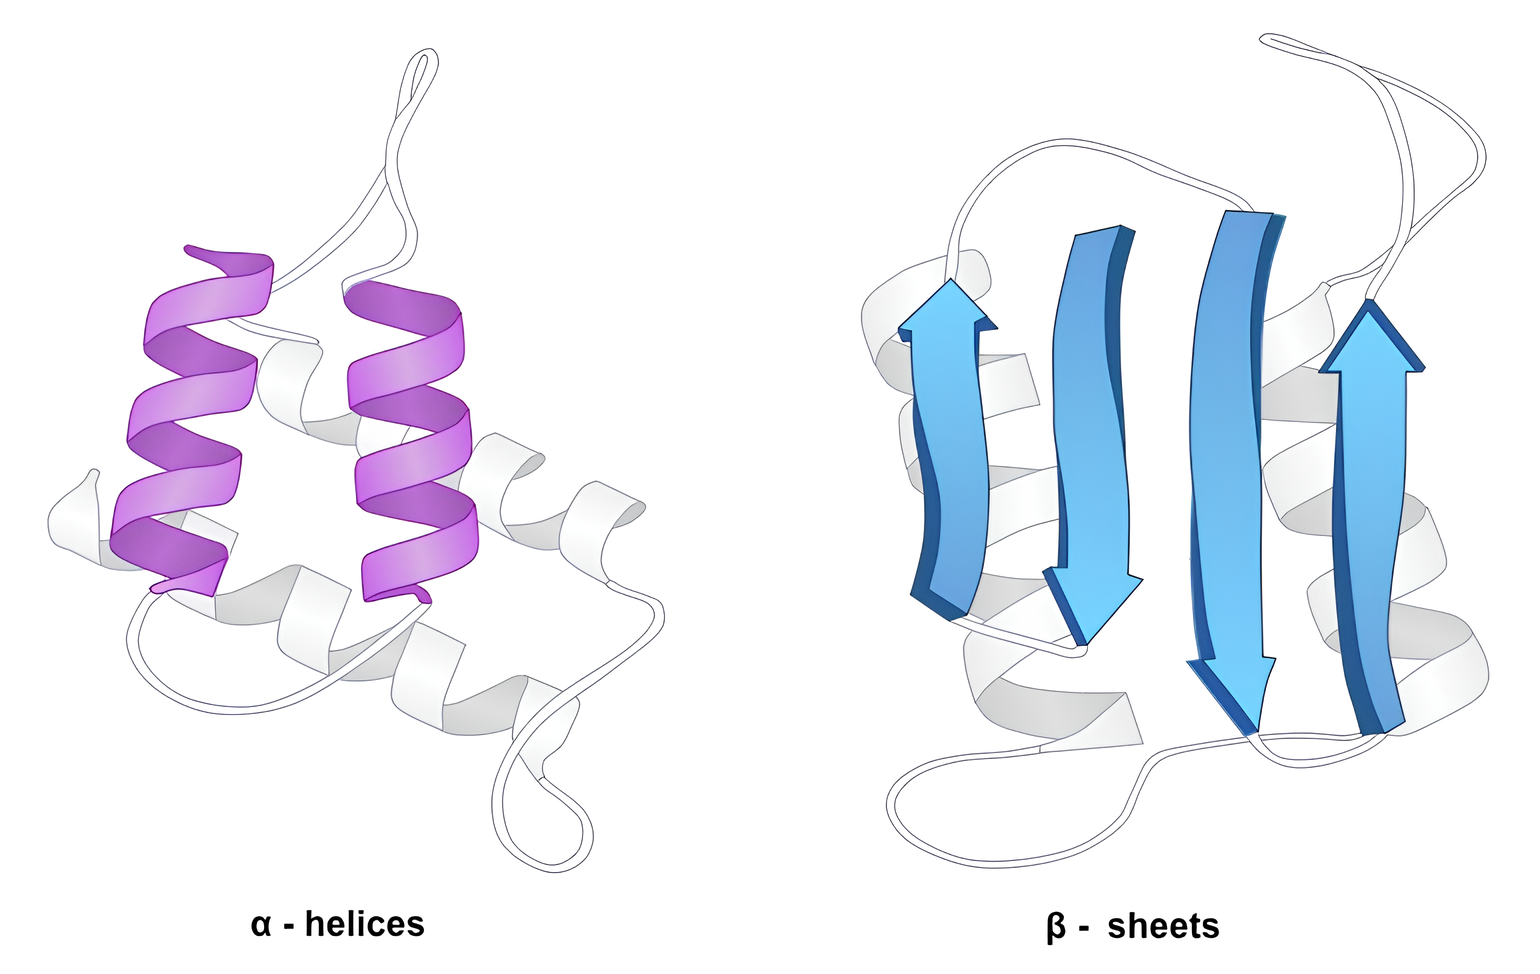
\includegraphics[width=0.8\textwidth]{img/ah_bs.png}
    \caption{Illustration of an alpha helix and a beta sheet, the two most common types of protein secondary structure. Generated with DALL·E 3.}
    \label{fig:alpha-beta}
\end{figure}

\xxx{TODO: change the picture}

The second level of protein structure is the \textbf{secondary structure}, which refers to local folding patterns within the polypeptide chain. The most common secondary structures are \textbf{alpha helices} and \textbf{beta sheets}, as shown in Figure~\ref{fig:alpha-beta}. These structures arise from hydrogen bonding between the backbone atoms of the amino acids, stabilizing the overall protein structure. All proteins also have a \textbf{three-dimensional (3D) structure}, also known as \textbf{tertiary structure}, which is crucial for their function \cite{nelson2008lehninger}, \cite{voet2010biochemistry}.

The secondary and tertiary structures are determined by the interactions between the side chains of the amino acids, including hydrophobic interactions, hydrogen bonds, ionic bonds, and disulfide bridges. The final level of protein structure is the \textbf{quaternary structure}, which refers to the assembly of multiple polypeptide chains into a functional protein complex \cite{nelson2008lehninger}, \cite{voet2010biochemistry}.

The tertiary and quaternary structures of proteins are determined through experimental methods such as X-ray crystallography and nuclear magnetic resonance (NMR) spectroscopy \cite{berman2000protein}. However, with the rise of deep learning and artificial intelligence, it is now also possible to predict protein structures from their amino acid sequences with remarkable accuracy. The most notable example is AlphaFold \cite{jumper2021highly}, \cite{abramson2024accurate}, a deep learning model developed by DeepMind that has achieved remarkable accuracy in predicting protein structures and has been widely adopted in the field of bioinformatics. AlphaFold also provides a per-residue confidence metric called the predicted Local Distance Difference Test (plDDT) score\footnotemark[1], which indicates the reliability of the predicted atomic positions. In recognition of the profound impact of these advances, the Nobel Prize in Chemistry was awarded in 2024 for the development of methods for the prediction of protein structures using artificial intelligence \cite{abriata2024nobel}. Other notable tools introduced in the past months include Boltz-2 \cite{passaro2025boltz2} and Chai-1 \cite{chai2024chai}. Today, predicted structures often closely match experimental results, as illustrated in Figure~\ref{fig:alphafold-vs-exp}.

\footnotetext[1]{The predicted Local Distance Difference Test (plDDT) score is a per-residue confidence metric output by AlphaFold, indicating the reliability of the predicted atomic positions; higher values suggest greater confidence. In the color scheme, blue indicates the most confident regions, while orange/yellow depict less confident regions.}

\begin{figure}[ht]
    \centering
    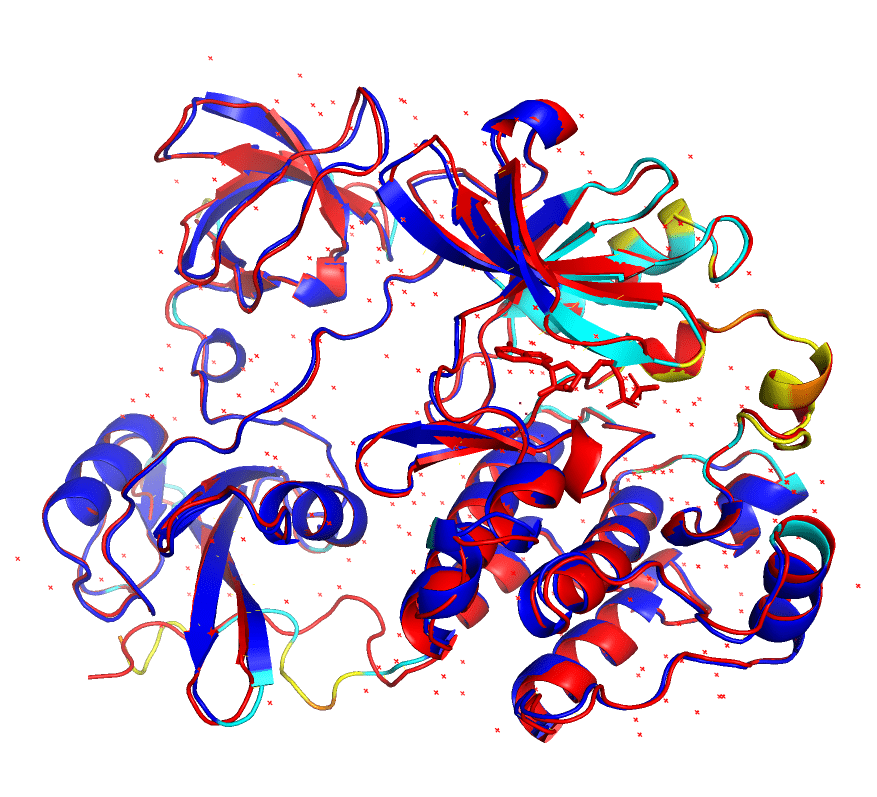
\includegraphics[width=0.8\textwidth]{img/alphafold_vs_exp.png}
    \caption{Comparison of AlphaFold predicted structure and experimental structure of the protein 2SRC (Crystal Structure of Human Tyrosine-Protein Kinase C-SRC, in Complex with AMP-PNP). The predicted structure is shown in blue to yellow colors (depicting the plDDT score), while the experimental structure is shown in red. The two structures are nearly identical after the alignment, demonstrating the accuracy of AlphaFold predictions. Image created in PyMOL.}
    \label{fig:alphafold-vs-exp}
\end{figure}
\par

Protein function is largely determined by interactions with other molecules, known as ligands. These may be small molecules, ions, RNA molecules, lipids, saccharides, or other molecules that bind to specific regions, often resulting in conformational changes that lead to different functions. Such interactions are crucial for processes like enzymatic catalysis, signal transduction, and immune response. In drug discovery, identifying and characterizing these sites is important, with computational approaches aiding both new therapeutic development and drug repurposing \cite{konc2019binding}. Additionally, de novo protein design allows for the creation of proteins with tailored functions, often guided by predictive tools such as AlphaFold before experimental testing \cite{huang2016coming}.

\section{Cryptic Binding Sites (CBSs)}
\label{sec:binding-sites}

\textbf{Binding sites} are distinct regions on a protein where ligands can bind and interact. These sites typically manifest as cavities or grooves on the protein surface and are frequently linked to conformational changes that influence protein function. Proteins with a ligand bound are termed \textbf{holo} conformations, while those lacking a ligand are called \textbf{apo} conformations. In holo conformations, the binding site is defined by the ligand’s position, whereas apo conformations may contain several potential binding sites, also commonly known as \textbf{pockets}.

\textbf{Cryptic binding sites (CBSs)} are regions on proteins that are not visible or accessible in the unbound (apo) structure but can form and become available for ligand binding following conformational changes. These sites typically appear only after ligand interaction or other molecular events that induce structural rearrangements. Computational methods such as CryptoBench \cite{vskrhak2025cryptobench} have been created to predict cryptic binding sites. A significant contribution in this area is CryptoSite \cite{cimermancic2016cryptosite}, which leverages known apo-holo protein pairs to identify CBSs, offering an alternative to time-consuming molecular dynamics simulations. Both of the methods will be covered in more detail in Section~\ref{sec:related-tools}.

\section{Databases and File Formats}
\label{sec:dbs-formats}

This section provides an overview of the key bioinformatics databases for protein structures and introduces the main file formats used in this field.

\subsection{PDB Archive and RCSB PDB}
\label{sec:rcsb-pdb}

The PDB (Protein Data Bank) Archive, often referred to simply as the "PDB database", is a comprehensive repository of 3D structural data for experimentally determined proteins, nucleic acids, and complex assemblies. It serves as a foundational resource for bioinformatics, with many machine learning and deep learning models relying on its data for training and validation. The archive is maintained by the wwPDB (Worldwide PDB) organization \cite{berman2003announcing}, which includes the RCSB PDB (Research Collaboratory for Structural Bioinformatics Protein Data Bank) \cite{berman2000protein}, PDBe (Protein Data Bank in Europe) \cite{velankar2010pdbe}, PDBj (Protein Data Bank Japan) \cite{kinjo2012protein}, and other members. 

The RCSB PDB (Research Collaboratory for Structural Bioinformatics Protein Data Bank) group offers a REST API for programmatic data access, which is publicly accessible at \url{https://www.rcsb.org/}. As of June 2025, the database contains over 238,000 structures.

Many organizations also maintain local, enriched copies of the PDB archive. The open sharing of structural data is encouraged, as it supports the development and improvement of computational models used throughout the scientific community \cite{callaway2025alphafold}.

\subsection{AlphaFold Database}
\label{sec:alphafold-db}

The AlphaFold Database \cite{varadi2024alphafold} contains over 200 million protein structures predicted by the AlphaFold model. While the majority of these structures have not been experimentally validated, those with high pLDDT scores are considered reliable. It is important to note that certain protein regions, known as intrinsically disordered regions, may exhibit low pLDDT scores due to their inherent flexibility and lack of stable structure. The database is publicly available at \url{https://alphafold.ebi.ac.uk/}.

\subsection{UniProt Database}
\label{sec:uniprot-db}

The UniProt database \cite{uniprot2025uniprot} is a comprehensive resource for protein sequences and functional information. Each protein is assigned a unique \textbf{UniProt accession} (also called \textbf{protein ID}), which serves as a standardized identifier for that specific protein. A single UniProt accession may correspond to multiple experimental structures in the PDB database, representing different conformations or states of the same protein, while typically having one predicted structure in the AlphaFold database. UniProt accessions are commonly used to link PDB and AlphaFold entries. UniProt is available at \url{https://www.uniprot.org/}. The main part of the UniProt database is the UniProt Knowledgebase (UniProtKB), which contains two sections: UniProtKB/Swiss-Prot, which includes manually curated entries with high-quality annotations, and UniProtKB/TrEMBL, which contains automatically annotated entries that have not yet been reviewed \cite{boutet2016uniprotkb}.

\subsection{PDB File Format}
\label{sec:pdb-format}

The PDB (Protein Data Bank) file format is a text-based format used to represent three-dimensional structures of biological molecules, primarily proteins and nucleic acids. It contains information about atom coordinates, connectivity, b-factors, and other structural details. Each PDB file should start with header lines providing metadata about the structure, such as the structure name, authors, methods used and additional comments. Then, the atomic coordinates are listed in a list of ATOM and HETATM records, which specify the atom type, residue name, chain identifier, residue sequence number, and the x, y, z coordinates of each atom in the structure. The PDB format might include information about secondary structure elements, such as helices and sheets \cite{westbrook2003pdb}. Some of the information might be ommited, especially in the case of working with structures generated by deep learning methods, such as RFDiffusion \cite{watson2023novo}. A single PDB file may contain multiple models representing distinct conformations of the same protein. It is worth noting that the PDB format is considered deprecated in favor of the more modern mmCIF format (covered in \ref{sec:mmcif-format}), though it remains widely used due to its simplicity and broad tool support.

\begin{figure}[H]
    \centering
    \lstinputlisting[caption={
        An edited example of a PDB file containing information about a protein structure generated by RFDiffusion.
    }]{code/rfdiff_example.pdb}
\end{figure}


\subsection{mmCIF File Format}
\label{sec:mmcif-format}

The mmCIF (Macromolecular Crystallographic Information File, also called PDBx) format is a more modern and flexible alternative to the PDB format, designed to overcome the limitations of the PDB format, especially for large structures \cite{bourne199730}. The PDB database, mentioned in Section~\ref{sec:rcsb-pdb}, has been transitioning to the mmCIF format for new entries. Although it is encouraged to use mmCIF for new structures, many existing tools and databases still rely on the PDB format thanks to its simpler format. Like PDB files, mmCIF files can also represent multiple conformations of the same structure.

\subsection{FASTA File Format}
\label{sec:fasta-format}

The FASTA file format is a widely used, text-based format for representing biological sequences, such as proteins or nucleic acids. Each sequence entry begins with a header line that starts with a ">" character, followed by a description or identifier. The sequence itself is written on the following lines, typically using single-letter codes. Multiple sequences can be included in a single FASTA file, each with its own header. While the header line is commonly present, it is technically optional, which allows easy creation of FASTA files \cite{lipman1985rapid}.

\begin{figure}[H]
    \centering
    \lstinputlisting[
        caption={
            An example of a FASTA file containing information about the 6A5J sequence (containing only 13 amino acids).
        },
        breaklines=true
    ]{code/fasta_example.fasta}
\end{figure}

\section{Related Tools, Projects}
\label{sec:related-tools}

This section is dedicated to the most relevant tools and projects important for the work presented in this thesis.

\subsection{P2Rank, PrankWeb}
\label{sec:prankweb-p2rank}

P2Rank is a Groovy/Java based standalone tool for predicting binding sites in protein structures. The P2Rank algorithm is based on machine learning. The structure is covered with a grid of points on the protein's solvent accessible surface, and each point is assigned a score based on the likelihood of being a binding site based on the local environment of the point. Then, the points are clustered and ranked based on their scores. The pre-trained tool does not rely on any external databases nor templates. The method is widely adapted due to its reliable and accurate predictions and speed \cite{krivak2018p2rank}. Source codes for P2Rank are available at \url{https://github.com/rdk/p2rank}.

PrankWeb is a web-based interface for P2Rank, allowing simple access to the P2Rank method without the need to run and install the tool locally. It is available at \url{https://prankweb.cz/}. The web interface allows users to upload a PDB/mmCIF file and receive a visualization of the prediction of the binding sites with the predicted binding sites colored according to their scores. Moreover, PrankWeb allows the users to perform molecular docking using the predicted binding sites, which is a common post-processing step in drug discovery \cite{polak2025prankweb}, \cite{jakubec2022prankweb}, \cite{jendele2019prankweb}. The docking is performed using the AutoDock Vina \cite{trott2010autodock} software, which is a widely used tool for molecular docking.

The PrankWeb interface was a huge inspiration for the design of the web interface presented in this thesis as the goal is to provide a similar user experience, but with a focus on cryptic binding sites and its specific challenges.

\subsection{AHoJ}
\label{sec:ahoj}

AHoJ (Apo–Holo Juxtaposition) is a web application for retreiving and visualizing apo-holo pairs of proteins (See Section~\ref{sec:binding-sites}). This functionality is useful especially for cryptic binding site predictions, as it allows the users to find similar structures with possibly similar properties based on the predicted CBS \cite{feidakis2022ahoj}. The application is available at \url{https://apoholo.cz/}. Currently, AHoJ supports searching for apo-holo pairs only by PDB ID.

AHoJ is integrated within the CryptoShow interface as well. This will be covered in more detail in Section~\ref{sec:trajectory}.

\subsection{PyMOL}
\label{sec:pymol}

PyMOL is a powerful molecular visualization tool written in Python. The users might use it either as a standalone application or as a Python library. Thanks to its feature-rich API and UI, PyMOL is a common choice for researchers in structural biology and cheminformatics \cite{delano2002pymol}.

\subsection{Mol*}
\label{sec:molstar}

Mol* (also MolStar) is a TypeScript library for visualizing molecular structures directly in web browsers. Thanks to its modern architecture, the usage of WebGL and rich feature set, Mol* is nowadays a very popular choice for web-based molecular visualization tools \cite{sehnal2018mol}. Mol* also provides an online version of a molecular viewer, which is available at \url{https://molstar.org/viewer/} \cite{sehnal2021mol}. A highly-customized version of the viewer is also used in the CryptoShow interface, which will be covered in more detail in Section~\ref{sec:frontend-molstar}.

\begin{figure}[ht]
    \centering
    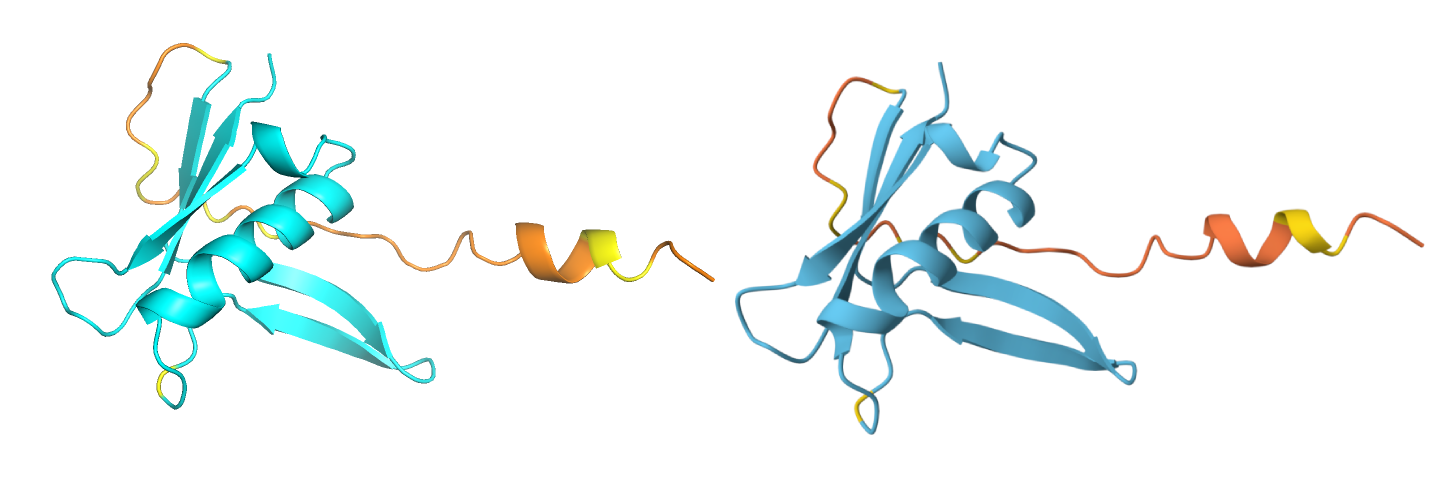
\includegraphics[width=\textwidth]{img/pymol-molstar.png}
    \caption{A comparsion of the PyMOL (left) and Mol* (right) molecular viewers showing the AlphaFold predicted structure of the protein AF\_AFQ9XWU9F1.}
    \label{fig:pymol-molstar}
\end{figure}

\subsection{CryptoBench}
\label{sec:cryptobench}

CryptoBench is a comprehensive benchmark dataset for training and evaluating CBSs prediction methods, built from a large set of apo–holo protein pairs and grouped by UniProt ID with predefined cross-validation splits. A part of the publication is dedicated to baseline evaluations, which show that a sequence-based neural network using protein language model embeddings outperforms state-of-the-art structure-based methods like PocketMiner \cite{meller2023predicting} and P2Rank \cite{krivak2018p2rank} across key metrics in terms of CBSs. The source codes for CryptoBench are available at \url{https://github.com/skrhakv/CryptoBench/} \cite{vskrhak2025cryptobench}.

The model used in CryptoBench (referred to as \textbf{CB-Model} in the context of this thesis) is able to predict cryptic binding sites when provided with ESM-2 embeddings \cite{lin2022language} of the protein sequence. The prediction capability represents one of the core functionalities of CryptoShow. More details about the CryptoBench method will be provided in Section~\ref{sec:prediction}.

\subsection{CryptoSite}
\label{sec:cryptosite}

CryptoSite is another tool designed to identify CBSs. By constructing a dataset of structurally defined apo–holo pairs, CryptoSite characterizes cryptic sites based on sequence, structure, and dynamics. Leveraging these insights, CryptoSite uses machine learning to predict cryptic sites with high accuracy, expanding the set of potentially druggable proteins. The tool has been applied to the human proteome, increasing the fraction of disease-associated proteins considered druggable. Experimental validation further demonstrates the practical use of CryptoSite. The web server is accessible at \url{https://modbase.compbio.ucsf.edu/cryptosite} \cite{cimermancic2016cryptosite}.

While CryptoSite is a valuable resource for cryptic binding site analysis and its web server remains available, its computational processes often take several days to complete, limiting its suitability for interactive use. In contrast, a primary goal of CryptoShow is to provide a fast and interactive experience, allowing users to obtain results within minutes. This need is underscored by the relatively low usage of CryptoSite; as of June 2025, only 10 jobs were submitted in the last 7 days. Also, the results of the CryptoSite jobs are available only for 7 days after the job completion.

\chapter{Methodology}
\label{chap:methodology}

In this chapter, we will cover the methodology used in this work. More details on the pipeline execution will be provided in Section \ref{sec:backend}.

\section{Prediction Using the CryptoBench Model, ESM-2}
\label{sec:prediction}

The initial step in our methodology involves utilizing the CryptoBench \cite{vskrhak2025cryptobench} model to generate residue-level predictions for protein sequences. It is important to note that this model works solely with sequence information, without incorporating any structural (tertiary or quaternary) data. Specifically, we employ the tiny variant of CryptoBench\footnote{Available at \url{https://github.com/skrhakv/TinyCryptobench}}, which is trained on a reduced version of the fine-tuned ESM-2 embeddings \cite{lin2022language} with 650 million parameters, as opposed to the full 3 billion. This choice is motivated by the observation that prediction accuracy remains comparable, while computational requirements are significantly reduced, enabling the pipeline to run efficiently on standard personal computers without the need for a GPU.

CryptoBench was created by filtering the AHoJ-DB \cite{feidakis2024ahoj} dataset, which contains a few million binding pockets. The filtering steps involved resolution filtering, removing redundant structures, geometric quality assurance, crypticity constraints, ligand filtering and sequence clustering. The final dataset consists of 1107 apo structures with 1361 cryptic binding sites. This dataset is used to train the model that has been benchmarked against PocketMiner \cite{meller2023predicting} and P2Rank \cite{krivak2018p2rank} and has shown better performance with the apo structures.

\sloppy
To begin with the prediction, the necessary dependencies for the CryptoBench model must be installed. Once the Python environment is set up, the fine-tuned ESM-2 model (\lstinline!facebook/esm2_t33_650M_UR50D!) is loaded, followed by the corresponding weight file from the Tiny-CryptoBench repository. The protein sequence is then tokenized using the ESM-2 tokenizer, segmented into chunks of 1022 tokens (1024 minus two special tokens), and processed by the CryptoBench model to obtain predictions. These predictions are subsequently concatenated to produce a single prediction vector representing the entire sequence.

\sloppy
The implementation for this procedure is provided in the \lstinline!backend/prediction/compute_score.py! file. The code is intended for use with individual protein sequences, as it requires parsing and splitting the sequence by chain to ensure accurate predictions.

This code is run asynchronously using Celery workers, allowing efficient processing of multiple sequences in parallel. Moreover, the implementation supports both GPU and CPU execution.

After the predictions are generated, the next step is to look for potential clusters of high-scoring residues and create the corresponding binding site candidates, as described in Section~\ref{sec:clustering}.

\section{Clustering and Smoothing}
\label{sec:clustering}

\xxx{TODO}

\section{Trajectory Animation}
\label{sec:trajectory}

\xxx{TODO}


\chapter*{Conclusion}
\addcontentsline{toc}{chapter}{Conclusion}


%%% Bibliography
%%% Bibliography (literature used as a source)
%%%
%%% We employ biblatex to construct the bibliography. It processes
%%% citations in the text (e.g., the \cite{...} macro) and looks up
%%% relevant entries in the bibliography.bib file.
%%%
%%% See also biblatex settings in thesis.tex.

%%% Generate the bibliography. Beware that if you cited no works,
%%% the empty list will be omitted completely.

% We let bibliography items stick out of the right margin a little
\def\bibfont{\hfuzz=2pt}

\printbibliography[heading=bibintoc]

%%% If case you prefer to write the bibliography manually (without biblatex),
%%% you can use the following. Please follow the ISO 690 standard and
%%% citation conventions of your field of research.

% \begin{thebibliography}{99}
%
% \bibitem{lamport94}
%   {\sc Lamport,} Leslie.
%   \emph{\LaTeX: A Document Preparation System}.
%   2nd edition.
%   Massachusetts: Addison Wesley, 1994.
%   ISBN 0-201-52983-1.
%
% \end{thebibliography}


%%% Figures used in the thesis (consider if this is needed)
\listoffigures

%%% Tables used in the thesis (consider if this is needed)
%%% In mathematical theses, it could be better to move the list of tables to the beginning of the thesis.
\listoftables

%%% Abbreviations used in the thesis, if any, including their explanation
%%% In mathematical theses, it could be better to move the list of abbreviations to the beginning of the thesis.
\chapwithtoc{List of Abbreviations}

%%% Doctoral theses must contain a list of author's publications
\ifx\ThesisType\TypePhD
\chapwithtoc{List of Publications}
\fi

%%% Attachments to the thesis, if any. Each attachment must be referred to
%%% at least once from the text of the thesis. Attachments are numbered.
%%%
%%% The printed version should preferably contain attachments, which can be
%%% read (additional tables and charts, supplementary text, examples of
%%% program output, etc.). The electronic version is more suited for attachments
%%% which will likely be used in an electronic form rather than read (program
%%% source code, data files, interactive charts, etc.). Electronic attachments
%%% should be uploaded to SIS. Allowed file formats are specified in provision
%%% of the rector no. 72/2017. Exceptions can be approved by faculty's coordinator.
\appendix
\chapter{Attachments}

\section{First Attachment}

\end{document}
